\documentclass{article}
\usepackage[utf8]{inputenc} %кодировка
\usepackage[T2A]{fontenc}
\usepackage[english,russian]{babel} %русификатор 
\usepackage{mathtools} %библиотека матеши
\usepackage[left=1cm,right=1cm,top=2cm,bottom=2cm,bindingoffset=0cm]{geometry} %изменение отступов на листе
\usepackage{amsmath}
\usepackage{graphicx} %библиотека для графики и картинок
\graphicspath{}
\DeclareGraphicsExtensions{.pdf,.png,.jpg}
\usepackage{subcaption}
\usepackage{pgfplots}
\usepackage{derivative}
\usepackage{amsfonts}


\begin{document}
% НАЧАЛО ТИТУЛЬНОГО ЛИСТА
\begin{center}
    \Large
    Федеральное государственное автономное \\
    образовательное учреждение высшего образования \\ 
    «Научно-образовательная корпорация ИТМО»\\
    \vspace{0.5cm}
    \large
    Факультет программной инженерии и компьютерной техники \\
    Направление подготовки 09.03.04 Программная инженерия \\
    \vspace{1cm}
    \Large
    \textbf{Отчёт по расчетно-графической работе №5} \\
    По дисциплине «Математический анализ» (третий семестр)\\
    \large
    \vspace{8cm}

    \begin{minipage}{.33\textwidth}
    \end{minipage}
    \hfill
    \begin{minipage}{.4\textwidth}
        \textbf{Группа}: \vspace{.1cm} \\
        \ МАТБАЗ 21.x\\ \\
        \textbf{Студенты}: \vspace{.1cm} \\
        \ Беляев Михаил\\
        \ Бутов Иван\\
        \ Дениченко Александр\\
        \ Разинкин Александр\\
        \ Хороших Дмитрий\\
        \\
        \textbf{Лектор}: \vspace{.1cm} \\
        \ Правдин Константин Владимирович \\ \\
        \textbf{Практик}:  \\
        \ Правдин Константин Владимирович
    \end{minipage}
    \vfill
Санкт-Петербург\\ 2023 г.
\end{center}

% КОНЕЦ ТИТУЛЬНОГО ЛИСТА
\newpage

\section*{Задание 3. Потенциал векторного поля}
Дано: векторное поле $\vec{H}$
\begin{equation*}
    \vec{H} = (e^x;-e^{y}) = e^x\cdot \overline{i}+(-e^y)\cdot\overline{j}
\end{equation*}
Решение:
\\ \\
1) Убедитесь, что данное векторное поле потенциально.

Чтобы доказать, что поле потенциально достаточно одного критерия. Векторное поле потенциально, если оно является градиентом некоторого скалярного поля. 
Необходимо и достаточно следующее:
\begin{equation*}
    rot(\vec{F}) = \overline{\nabla}\text{ x }\vec{F} = 
    \begin{vmatrix}
        \overline{i}&\overline{j}&\overline{k}\\
        \pdv{}{x}&\pdv{}{y}&\pdv{}{z}\\
        P&Q&R\\
    \end{vmatrix}
    = 0
\end{equation*}
\begin{equation*}
    rot(\vec{H}) = \overline{\nabla}\text{ x }\vec{H} = 
    \begin{vmatrix}
        \overline{i}&\overline{j}&\overline{k}\\
        \pdv{}{x}&\pdv{}{y}&\pdv{}{z}\\
        P&Q&R\\
    \end{vmatrix}
    = \overline{i}(0-0) + \overline{j}(0-0) + \overline{k}(0-0)
    = 0
\end{equation*}
Поле потенциально (безвихриво).
\\
\\
2) Найдите уравнения векторных линий. Изобразите векторные линии на рисунке.

Векторные линии можно найти следующим способом:
\begin{equation*}
    tg\alpha = y' = \frac{Q}{P}
\end{equation*}
\begin{equation*}
    y' = \frac{-e^y}{e^x}
\end{equation*}
После решения ДУ, получили уравнение векторных линий:
\begin{equation*}
    y = ln\left(\frac{e^x}{Ce^x-1}\right),\ C\in \mathbb{R}
\end{equation*}
Векторные линии поля на графике:
\begin{center}
    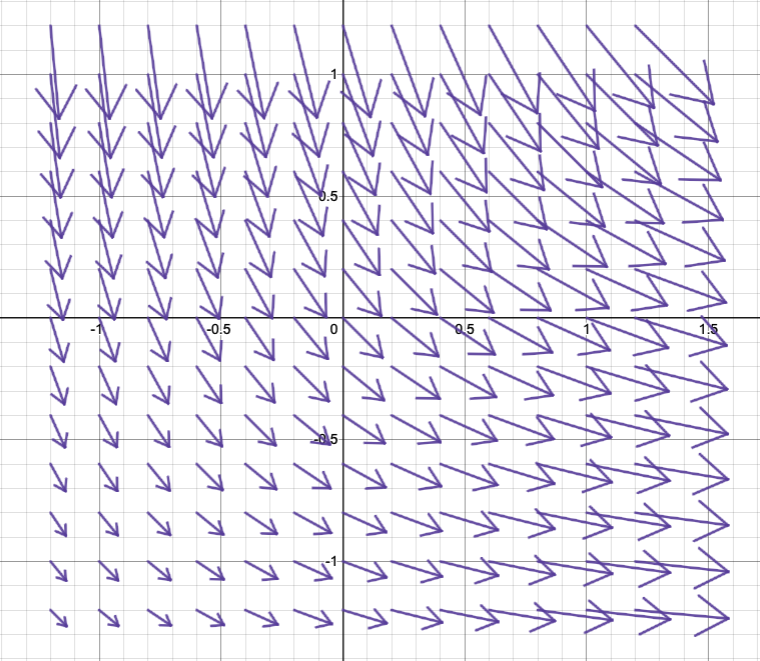
\includegraphics[width=.5\textwidth]{vecLin.png}
\end{center}
3) Найдите потенциал поля при помощи криволинейного интеграла.
\begin{equation*}
    \mathbb{U}(x, y) = \int_{AB}Pdx+Qdy = \int_{x_0}^{x}P(x, y)dx +\int_{y_0}^{y}Q(x, y)dx
\end{equation*}
\begin{equation*}
    \mathbb{U}(x, y) = \int_{x_0}^{x}e^xdx -\int_{y_0}^{y}e^ydx = e^x-e^y-e^{x_0}+e^{y_0}
\end{equation*}
Проверка:
\begin{equation*}
    grad(\mathbb{U}) = \vec{H} = \pdv{\mathbb{U}}{x} + \pdv{\mathbb{U}}{y}
\end{equation*}
\begin{equation*}
    \pdv{\mathbb{U}}{x} = e^x
\end{equation*}
\begin{equation*}
    \pdv{\mathbb{U}}{y} = -e^y
\end{equation*}
\begin{equation*}
    grad(\mathbb{U}) = \vec{H} = e^x -e^y
\end{equation*}
\\
4) Найдите уравнения линий уровня потенциала (эквипотенциальных линий). Изобразите
линии уровня потенциала.

Существует такая $f$, что:
\begin{equation*}
    \nabla f = \vec{H}
\end{equation*}
Тогда:
\begin{equation*}
    \pdv{f(x,y)}{x} = e^x;\ f(x,y) = \int e^xdx = e^x + C(y)
\end{equation*}
\begin{equation*}
    \pdv{f(x,y)}{x} = -e^y;\ f(x,y) = \int -e^ydx = -e^y + C_1
\end{equation*}
\begin{equation*}
    f(x, y) = e^x - e^y + C_1
\end{equation*}
Линии уровня:
\begin{equation*}
    f(x, y) = C_2
\end{equation*}
\begin{equation*}
    e^x - e^y = C\
\end{equation*}
\begin{equation*}
    y = ln(e^x-C)
\end{equation*}
Линии уровня потенциала:
\begin{center}
    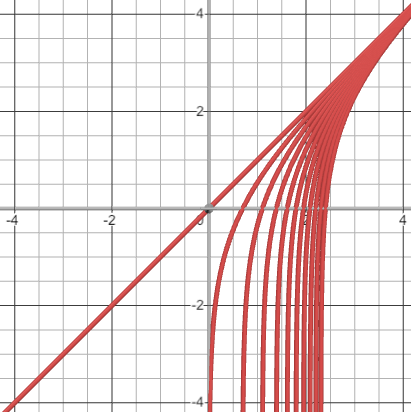
\includegraphics[width=.5\textwidth]{linU.png}
\end{center}
5) Докажите ортогональность найденных векторных линий поля и линий уровня потенциала.
Проиллюстрируйте ортогональность на графике.

Докажем ортогональность для
\begin{equation*}
    y_u = ln(e^x-C_1); \ y_v = ln\left(\frac{e^x}{C_2e^x-1}\right)
\end{equation*}
Зафиксируем точку $C = C_1 = C_2$ и найдём производные:
\begin{equation*}
    y_u' = \frac{e^x}{e^x-C}; \ y_v' = -\frac{1}{Ce^x-1}
\end{equation*}
Произведение производных в точне пересечения, которую определяет в первую очередь параметр C, должно быть равно -1. Покажем общую формулу, где предположим, что $x=x_0$
\begin{equation*}
    y_u'\cdot y_v' =(\frac{e^{x_0}}{e^{x_0}-C})\cdot (-\frac{1}{Ce^{x_0}-1}) = - \frac{e^{x_0}}{Ce^{2x_0}-e^{x_0}-C^2e^{x_0}+C}
\end{equation*}
Пусть фиксированная C = 1, тогда точка пересечения:
\begin{equation*}
    e^x-e^{ln(\frac{e^x}{e^x-1})} = 1
\end{equation*}
\begin{equation*}
    x= ln\left(\frac{3+\sqrt{5}}{2}\right)
\end{equation*}
Подставим эту точку:
\begin{equation*}
    y_u'\cdot y_v' = - \frac{e^{ln\left(\frac{3+\sqrt{5}}{2}\right)}}{e^{2ln\left(\frac{3+\sqrt{5}}{2}\right)}-e^{ln\left(\frac{3+\sqrt{5}}{2}\right)}-e^{ln\left(\frac{3+\sqrt{5}}{2}\right)}+1} = -1
\end{equation*}
Проиллюстрируем ортогональность на графике.
\begin{center}
    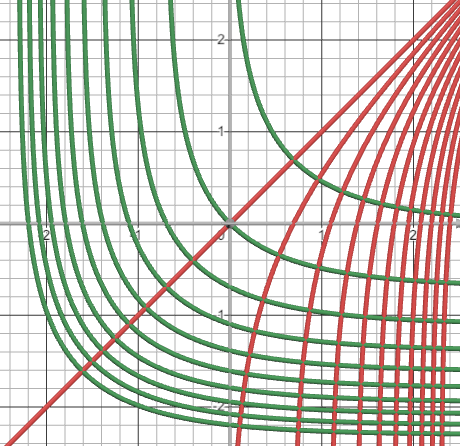
\includegraphics[width=.5\textwidth]{double.png}
\end{center}
6) Выберите какую-либо векторную линию поля и зафиксируйте на ней точки A и B, выбрав
для них числовые координаты. Вычислите работу поля вдоль этой линии, используя найденный в п. 3) потенциал.

Работа потенциального поля по кривой AB:
\begin{equation*}
    A = \int_{A}^{B}\vec{H}\cdot d\overline{l} = \mathbb{U}(B) - \mathbb{U}(A)
\end{equation*}
Фиксируем точки B(-2;0), A(0;-2), тогда:
\begin{equation*}
    A = e^{-2}-e^{0}-e^{0}+e^{-2} = -1,73 \text{ Дж}
\end{equation*}
\section*{Задание 4. Поток векторного поля}
Дано: Дано тело Т, ограниченное следующими поверхностями:
\begin{equation*}
    y+\sqrt{x^2+z^2}=0
\end{equation*}
\begin{equation*}
    x^2+y^2=1
\end{equation*}
\begin{equation*}
    x^2+y+z^2=2
\end{equation*}
На рисунке представлено сечение тела Т координатной плоскостью Oyz.
\begin{center}
    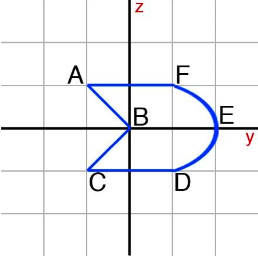
\includegraphics[width=.3\textwidth]{figure.png}
\end{center}
Решение:
\\ \\
1) Изобразите тело Т на графике в пространстве.
\begin{center}
    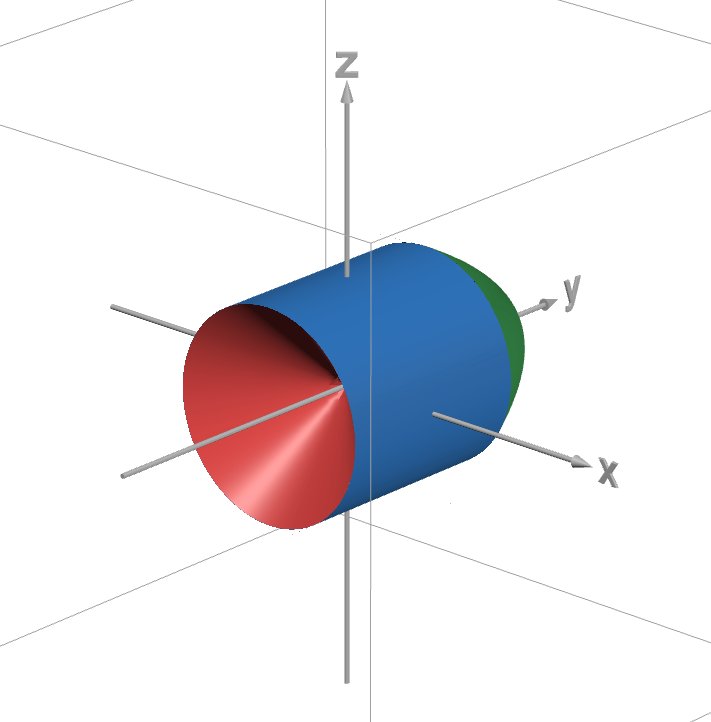
\includegraphics[width=.5\textwidth]{top.png}
\end{center}
\begin{center}
    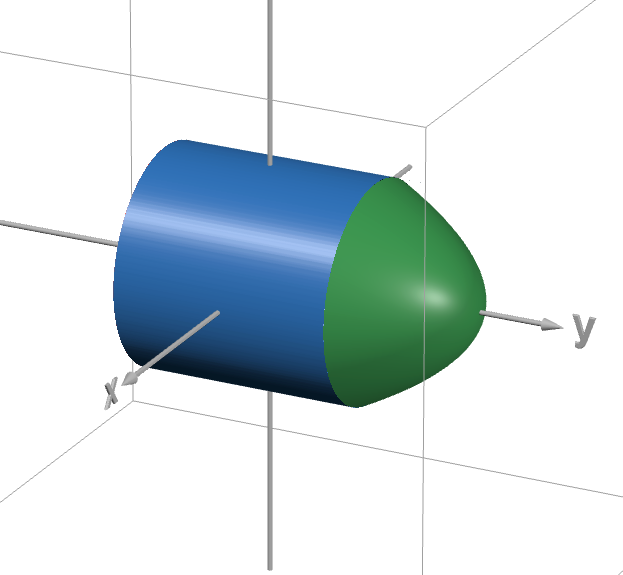
\includegraphics[width=.5\textwidth]{button.png}
\end{center}
2) Вычислите поток поля $a=(sin\ zy^2)\vec{i}+ \sqrt{2}x\vec{j}+(\sqrt{2+y}-3z)\vec{k}$ через боковую
поверхность тела T, образованную вращением дуги AFEDC вокруг оси Oy, в направлении внешней нормали поверхности тела Т.

\begin{equation*}
    \iint_{S^+}\vec{a}\cdot d\vec{S}=\iiint_Tdiv\vec{a}\cdot dV =
    \iiint_T(\pdv{sin\ zy^2}{x}+\pdv{\sqrt{2}x}{y}+\pdv{\sqrt{2+y}-3z}{z})dxdydz =
\end{equation*}
Перейдём в цилиндрическую систему координат:
\begin{equation*}
    y=y;\ x=\rho cos\phi;\ z=\rho sin\phi; |\mathbb{J}|=\rho
\end{equation*}
\begin{equation*}
    \rho^2cos^2\phi+y+\rho^2sin^2\phi =2;\ y+\rho^2=2;\ \rho^2=2-y;\ \rho = \sqrt{2-y}
\end{equation*}
\begin{equation*}
    \text{Первая фигура: }
    \begin{cases}
        -1\leq y\leq 1\\
        0\leq\rho \leq 1\\
        0\leq \phi < 2\pi
    \end{cases}
    \text{Вторая фигура: }
    \begin{cases}
        1< y\leq 2\\
        0\leq\rho \leq \sqrt{2-y}\\
        0\leq \phi < 2\pi
    \end{cases}
\end{equation*}
\begin{equation*}
    =-3\iiint_Tdxdydz = -3(\int_{-1}^{1}dy\int_{0}^{2\pi}d\phi\int_{0}^{1}\rho d\rho+\int_{1}^{2}dy\int_{0}^{2\pi}d\phi\int_{0}^{\sqrt{2-y}}\rho d\rho)=-3\pi(1-(-1)+(2\cdot 2-\frac{1}{2}\cdot 2^2-(2\cdot 1-\frac{1}{2}\cdot 1)))=
\end{equation*}
\begin{equation*}
    =-\frac{15}{2}\pi
\end{equation*}
\end{document}


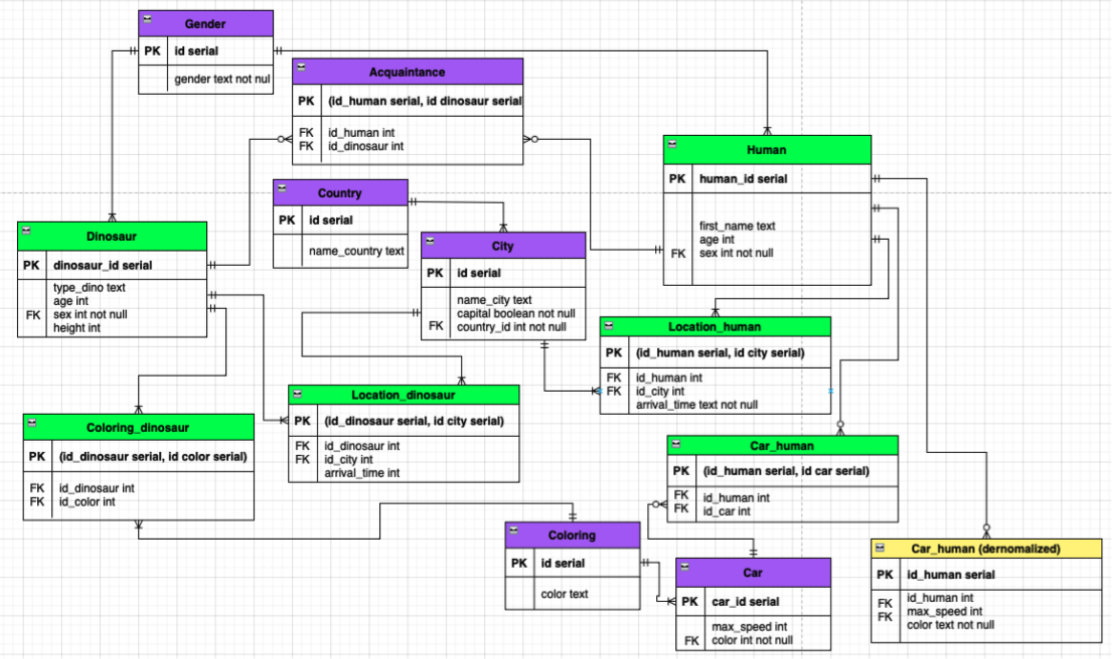
\includegraphics[width=.9\textwidth]{123}